\def\cellWidth{1.5}
\def\cellHeight{5}

\def\cellPosWidth{0.5}
\def\cellPosHeight{0.1}

\ctikzsubcircuitdef{spiccell} {
    north, south, east, west,
    northeast, northwest, southeast, southwest,
    center,
    p, n%
} {
    coordinate (#1-origin)
    ++({\cellWidth/2},{(-\cellHeight-\cellPosHeight)/2})
    node [inner sep = 0pt, anchor = center] {
        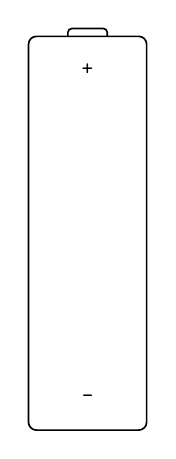
\begin{tikzpicture}
            \draw [semithick, rounded corners = 1mm]
            (0,0) coordinate (origin)
            (origin) rectangle ++(\cellWidth,-\cellHeight)
            ;
            \draw [semithick, rounded corners = 0.5mm]
            (origin) ++({(\cellWidth/2)-(\cellPosWidth/2)},0)
            -- ++(0,\cellPosHeight)
            -- ++(\cellPosWidth,0)
            -- ++(0,-\cellPosHeight)
            ;
            \draw
            (origin) ++({\cellWidth/2},0)
            coordinate (mid) ++(0,-0.25)
            node [below = 0pt, scale = 0.8] {\texttt{+}}
            (mid) ++(0,{-\cellHeight+0.25})
            node [above = 0pt, scale = 0.8] {\texttt{-}}
            ;
        \end{tikzpicture}
    }
    (#1-origin) ++({\cellWidth/2},0) coordinate (#1-p)
    ++(0,{-\cellHeight-\cellPosHeight}) coordinate (#1-n)
    \markgeocoordinate {#1}
    {(#1-origin)} {
        (#1-origin) ++({\cellWidth},{(-\cellHeight-\cellPosHeight)})
    }
    {(#1-origin)} {
        (#1-origin) ++({\cellWidth},{(-\cellHeight-\cellPosHeight)})
    }
}

\ctikzsubcircuitactivate{spiccell}
